\documentclass[letterpaper,12pt]{article}

\usepackage{tabularx} % extra features for tabular environment
\usepackage{amsmath}  % improve math presentation
\usepackage{graphicx} % takes care of graphic including machinery
\usepackage[margin=1in,letterpaper]{geometry} % decreases margins
\usepackage[final]{hyperref} % adds hyper links inside the generated pdf file
\usepackage{ctex}
\usepackage{titlesec}
%\usepackage{CJKutf8, CJK}
\usepackage{makecell}                 % 三线表-竖线
\usepackage{booktabs}                 % 三线表-短细横线
% \usepackage{natbib}
\usepackage{graphicx}				  % 表格单元格逆时针
\usepackage{multirow}				  % 合并单元格
\usepackage{array}
\usepackage{amssymb}				  % 勾
\usepackage{amsmath}
\usepackage{longtable}                % 导入 longtable 宏包,表格自动换行
\usepackage{caption}
\usepackage{subcaption}               % 设置子图
\usepackage{color}					  % 文本颜色包
\usepackage{xcolor}
\usepackage{bbm}					  % 输入指示函数
\usepackage{tablefootnote}			  % 表格注释
\usepackage{pythonhighlight}
\usepackage{fancyhdr}
\usepackage{lastpage}
\pagestyle{fancy}
\fancyhf{}
\fancyhead{}
\fancyfoot{}
\fancyhead[R]{\small Page \thepage\ of \pageref*{LastPage}}
\fancyhead[L]{\small Assignment: Self-Attention, Transformers, and Pretraining}
\usepackage{listings}                 % 导入代码块
\usepackage{xcolor}
\lstset{
	numbers=none, 
	tabsize=1,
	columns=flexible, 
	%numberstyle=  \small, 
	%keywordstyle= \color{blue!70},
	commentstyle= \color{green!50!blue!100}, 
	%frame=shadowbox, % 阴影效果
	frame=tlrb
	rulesepcolor= \color{red!20!green!20!blue!20} ,
	%escapeinside=``, % 英文分号中可写入中文
	%xleftmargin=2em,
	%xrightmargin=2em, 
	aboveskip=1em,
} 

\hypersetup{
	colorlinks=true,       % false: boxed links; true: colored links
	linkcolor=blue,        % color of internal links
	citecolor=blue,        % color of links to bibliography
	filecolor=magenta,     % color of file links
	urlcolor=blue       
}

%++++++++++++++++++++++++++++++++++++++++
\titleformat{\section}{\large\bfseries\songti}{\thesection}{1em}{}
\titleformat{\subsection}{\large\bfseries\songti}{\thesubsection}{1em}{}
\titleformat{\subsubsection}{\normalsize\bfseries\songti}{\thesubsubsection}{1em}{}
\titleformat{\paragraph}{\small\bfseries\songti}{\paragraph}{1em}{}
\titleformat{\subparagraph}{\footnotesize\bfseries\songti}{\subparagraph}{1em}{}

\begin{document}

	
	\renewcommand{\figurename}{Figure} % 可以重新定义abstract,因为ctex会覆盖thebibliography
	% 	\begin{abstract}
		%		In this experiment we studied a very important physical effect by measuring the
		%		dependence of a quantity $V$ of the quantity $X$ for two different sample
		%		temperatures.  Our experimental measurements confirmed the quadratic dependence
		%		$V = kX^2$ predicted by Someone's first law. The value of the mystery parameter
		%		$k = 15.4\pm 0.5$~s was extracted from the fit. This value is
		%		not consistent with the theoretically predicted $k_{theory}=17.34$~s. We attribute %this
		%		discrepancy to low efficiency of our $V$-detector.
		%	\end{abstract}
	\renewcommand{\contentsname}{Contents}
	\renewcommand{\tablename}{Table}
	
	\section{Attention exploration (22 points)}
	
	\noindent Multi-headed self-attention is the core modeling component of Transformers. In this question, we'll get some practice working with the self-attention equations, and motivate why multi-headed self-attention can be preferable to single-headed self-attention.
	Recall that attention can be viewed as an operation on a \textit{query} $q \in \mathbb{R}^d$, a set of \textit{value} vectors $\{v_1, . . . , v_n \}$, $v_i \in \mathbb{R}^d$, and a set of \textit{key} vectors $\{k_1, . . . , k_n\}$, $k_i \in \mathbb{R}^d$, specified as follows:
	
	\begin{equation}
		\begin{aligned}
			c = \sum_{i=1}^{n} v_{i}\alpha_{i}
		\end{aligned}
		\label{eq: Attention_formula_1}
	\end{equation}
	
	\begin{equation}
		\begin{aligned}
			\alpha_{i} = \frac{\exp(k_{i}^{T}q)}{\sum_{j=1}^{n} \exp(k_{j}^{T}q)}
		\end{aligned}
		\label{eq: Attention_formula_2}
	\end{equation}
	with $\alpha_i$ termed the "attention weights". Observe that the output $c \in \mathbb{R}^d$ is an average over the value vectors weighted with respect to $\alpha_i$.

	\noindent(a) (4 points) \textbf{Copying in attention.} One advantage of attention is that it's particularly easy to "copy" a value vector to the output $c$. In this problem, we'll motivate why this is the case.
		
	\begin{itemize}
	\item [i.]
	(1 point) \textbf{Explain} why $\alpha$ can be interpreted as a categorical probability distribution.
			
	\textcolor{blue!70}{\textbf{Answer:} There are n $\alpha$ scores, each corresponding to a value in a sequence. These scores range from 0 to 1 and can be viewed as probabilities. The scores collectively form a distribution since they are normalized, meaning that their sum totals to 1.}

	\item [ii.]
	(2 points) The distribution $\alpha$ is typically relatively "diffuse"; the probability mass is spread out between many different $\alpha_i$. However, this is not always the case. \textbf{Describe} (in one sentence) under what conditions the categorical distribution $\alpha$ puts almost all of its weight on some $\alpha_j$ , where $j \in \{1, \ldots , n\} (i.e. \quad \alpha_j \gg \sum_{i\neq j} \alpha_i)$. What must be true about the query $q$ and/or the keys $\{k_1, \ldots , k_n\}$?
			
	\textcolor{blue!70}{\textbf{Answer:} When the key values $k_j$ are significantly larger compared to other key values $k_{i\neq j}$ (i.e., $k_j \gg k_i$, for $i \in {1,\ldots, n}$ and $i \neq j$), the dot product between the key and the query will be large as well. As a result, the softmax function will assign a higher probability to the large value, concentrating most of its probability mass on that particular key value.}

	\item [iii.]
	(1 point) Under the conditions you gave in (ii), \textbf{describe} what properties the output c might have.
			
	\textcolor{blue!70}{\textbf{Answer:} The $j^{th}$ value will be assigned the highest weight, resulting in a similarity between $c$ and $v_j$, denoted as $c \approx v_j$.}

    \item [iv.]
	(1 point) \textbf{Explain} (in two sentences or fewer) what your answer to (ii) and (iii) means intuitively.
			
	\textcolor{blue!70}{\textbf{Answer:} When the dot product (similarity) between the key of a particular word (indexed as $j$) and a given query is significantly larger than the dot products of other words' keys with the same query, the attention output for that word ($j$) will converge towards its corresponding value. In other words, it can be interpreted as if the value is effectively "transferred" or "replicated" to the output.}
	\end{itemize}	
		
	\noindent(b) (7 points) \textbf{An average of two}. Instead of focusing on just one vector $v_j$ , a Transformer model might want to incorporate information from \textit{multiple} source vectors. Consider the case where we instead want to incorporate information from \textbf{two} vectors $v_a$ and $v_b$, with corresponding key vectors $k_a$ and $k_b$.
	
	\begin{itemize}
	\item [i.]
	(3 points) How should we combine two d-dimensional vectors $v_a$, $v_b$ into one output vector $c$ in a way that preserves information from both vectors? In machine learning, one common way to do so is to take the average:  $c = \frac{1}{2}(v_a + v_b)$. It might seem hard to extract information about the original vectors va and $v_b$ from the resulting $c$, but under certain conditions one can do so.
	In this problem, we'll see why this is the case.
			
	\vspace{1em}
			
	Suppose that although we don't know $v_a$ or $v_b$, we do know that $v_a$ lies in a subspace $A$ formed by the $m$ basis vectors $\{a_1, a_2, \ldots , a_m\}$, while $v_b$ lies in a subspace $B$ formed by the $p$ basis vectors $\{b_1, b_2, \ldots , b_p\}$. (This means that any va can be expressed as a linear combination of its basis vectors, as can $v_b$. All basis vectors have norm 1 and orthogonal to each other.)
			
	Additionally, suppose that the two subspaces are orthogonal; i.e. $a^\top_j b_k = 0$ for all $j$, $k$.
	Using the basis vectors $\{a_1, a_2, \ldots , a_m\}$, construct a matrix $M$ such that for arbitrary vectors $v_a \in A$ and $v_b \in B$, we can use $M$ to extract $v_a$ from the sum vector $s = v_a + v_b$. In other words, we want to construct $M$ such that for any $v_a$, $v_b$, $M_s = v_a$.
			
	\textbf{Note:} both $M$ and $v_a$, $v_b$ should be expressed as a vector in $\mathbb{R}^d$, not in terms of vectors from $A$ and $B$.
			
	\textbf{Hint:} Given that the vectors $\{a_1, a_2, \ldots , a_m\}$ are both \textit{orthogonal} and \textit{form a basis} for $v_a$, we know that there exist some $c_1, c_2, \ldots , c_m$ such that $v_a = c_1a_1 + c_2a_2 + \ldots + c_ma_m$. Can you create a vector of these weights $c$?
			
	\textcolor{blue!70}{\textbf{Answer:} Let's consider matrices $A$ and $B$, which contain concatenated basis vectors $\{a_1, a_2,\ldots, a_m\}$ and $\{b_1, b_2,\ldots, b_p\}$, respectively. We want to find a matrix $M$ that satisfies the following conditions: when multiplied with vector $v_b$, it results in the zero vector, and when multiplied with vector $v_a$, it produces the same vector $v_a$ in terms of its own space.
	By observing the properties of the basis vectors, we can see that $A^\top B$ = 0 since the dot product of any $a_i$ and $b_j$ is zero for all $i$ and $j$. Additionally, $A\top A = I$ (the identity matrix) because the dot product of ai with $a_j$ equals 0 when $i \neq j$, and it equals 1 when $i = j$ due to the normalization of the vectors.
	Now, if we substitute $M$ with $A^\top$ in the equation $$Mv_a + Mv_b = v_a$$, we get $$A^\top Ac + A^\top Bd = Ic + 0d = c$$. This means that when we multiply $A^\top$ with vector $v_a$, we obtain the original vector $c$.
	Therefore, we can conclude that $$M = A^\top$$ satisfies the desired conditions and produces the same result as vector $v_a$ in terms of its own space ($\mathbb{R}^d$), without explicitly referring to matrices $A$ and $B$.
	} 
			
			
	\item[ii.]
	(4 points) As before, let $v_a$ and $v_b$ be two value vectors corresponding to key vectors $k_a$ and $k_b$, respectively. Assume that (1) all key vectors are orthogonal, so $k_i^\top k_j$ for all $i \neq j$; and (2) all key vectors have norm 1.\footnote{Recall that a vector x has norm 1 if $x^{\top}x = 1$.} \textbf{Find an expression} for a query vector $q$ such that $c \approx \frac{1}{2}(v_a +v_b)$.\footnote{Hint: while the softmax function will never exactly average the two vectors, you can get close by using a large scalar multiple in the expression.}
	
	\textcolor{blue!70}{\textbf{Answer:} Assume that $c$ is approximated as follows:
	\begin{equation*}
		\begin{aligned}
			c \approx \frac{1}{2}\mathbf{v}_a + \frac{1}{2}\mathbf{v}_b
		\end{aligned}
	\end{equation*}
	This means we want $\alpha_a \approx 0.5$ and $\alpha_b \approx 0.5$, which can be achieved when (whenever $i \neq a$ and $i \neq b$):
	\begin{equation*}
		\begin{aligned}
			\mathbf{k}_a^\top q \approx \mathbf{k}_b^\top q \gg \mathbf{k}_i^\top \mathbf{q}
		\end{aligned}
	\end{equation*}
	Like explained in the previous question, if the dot product is big, the probability mass will also be big and we want a balanced mass between $\alpha_a$ and $\alpha_b$. $q$ will be largest for $k_a$ and $k_b$ when it is a large multiplicative of a vector that contains a component in $k_a$ direction and in $k_b$ direction:
	\begin{equation*}
		\begin{aligned}
			\mathbf{q} = \beta (\mathbf{k}_a + \mathbf{k}_b), \quad \text{where} \beta \gg 0
		\end{aligned}
	\end{equation*}
	Now, since the keys are orthogonal to each other, it is easy to see that:
	\begin{equation*}
		\begin{aligned}
			\mathbf{k}_a^\top q = \beta; \mathbf{k}_b^\top q = \beta; \mathbf{k}_i^\top q = 0, \quad \text{whever} \ i\neq a \ \text{and} \ i\neq b
		\end{aligned}
	\end{equation*}
	Thus when we exponentiate, only $\exp(\beta)$ will matter, because $\exp(0)$ will be insignificant to the probability mass. We get that:
	\begin{equation*}
		\begin{aligned}
			\alpha_a=\alpha_b=\frac{\exp(\beta)}{n-2+2\exp(\beta)} \approx \frac{\exp(\beta)}{2\exp(\beta)} \approx \frac{1}{2}, \ \text{for} \ \beta \gg 0
		\end{aligned}
	\end{equation*}
	}
	
	\end{itemize}	
	
	
	
	\noindent(c) (5 points) \textbf{Drawbacks of single-headed attention:} In the previous part, we saw how it was \textit{possible} for a single-headed attention to focus equally on two values. The same concept could easily be extended to any subset of values. In this question we'll see why it's not a practical solution. Consider a set of key vectors $\{k_1, \ldots , k_n\}$ that are now randomly sampled, $k_i \sim \mathcal{N}(μ_i,\Sigma_i)$, where the means $μ_i \in \mathbb{R}^d$ are known to you, but the covariances $\Sigma_i$ are unknown. Further, assume that the means $μ_i$ are all perpendicular; $\mu^\top_i \mu_j = 0$ if $i \neq j$, and unit norm, $\|\mu_i\| = 1$.
	
	\begin{itemize}
	\item[i.]
		(2 points) Assume that the covariance matrices are $\Sigma_i = \alpha I \forall i \in {1, 2, \ldots , n}$, for vanishingly small $\alpha$. Design a query $q$ in terms of the $\mu_i$ such that as before, $c \approx \frac{1}{2}(v_a +v_b)$, and provide a brief argument as to why it works.
		
		\textcolor{blue!70}{\textbf{Answer:} Because the covariance matrix is small, $k_i$ can be approximately replaced by $\mu_i$:
		\begin{equation*}
			\begin{aligned}
				k_i \approx \mu_i
			\end{aligned}
		\end{equation*}
		Since the key vectors $k_a$ and $k_b$ are orthogonal to each other, the problem can be reduced to the previous case where all keys were orthogonal. Therefore, the expression for the query vector $q$ remains the same as in the previous case: 
		\begin{equation*}
			\begin{aligned}
				\mathbf{q}=\beta(\mu_a+\mu_b), \quad \text{where} \ \beta \gg 0
			\end{aligned}
		\end{equation*}
		}
		
	\item[ii.]
		(3 points) Though single-headed attention is resistant to small perturbations in the keys, some types of larger perturbations may pose a bigger issue. Specifically, in some cases, one key vector $k_a$ may be larger or smaller in norm than the others, while still pointing in the same direction as $\mu_a$. As an example, let us consider a covariance for item $a$ as $\Sigma_a = \alpha I+ \frac{1}{2}(\mu_a\mu^\top_a )$ for vanishingly small $\alpha$ (as shown in Fig. \ref{fig: vector}). This causes $k_a$ to point in roughly the same direction as $\mu_a$, but with large variances in magnitude. Further, let $\Sigma_i = \alpha I$ for all $i \neq a$.
		
		\begin{figure}[htbp] 
			% read manual to see what [ht] means and for other possible options
			\centering 
			% \includegraphics[width=0.8\columnwidth]{GLADNet}
			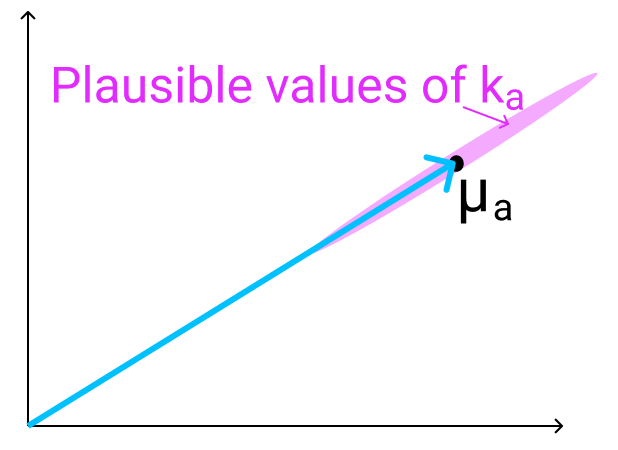
\includegraphics[width=0.5\linewidth]{picture/ka_plausible}
			\captionsetup{font=small}
			\label{vector}
			\caption{
				\label{fig: vector} % spaces are big no-no withing labels
				% things like fig: are optional in the label but it helps
				% to orient yourself when you have multiple figures,
				% equations and tables
				The vector $\mu_a$ (shown here in 2D as an example), with the range of possible values of $k_a$ shown in red. As mentioned previously, $k_a$ points in roughly the same direction as $\mu_a$, but may have larger or smaller magnitude.
			}
		\end{figure}
		
		When you sample $\{k_1, \ldots , k_n\}$ multiple times, and use the $q$ vector that you defined in part i., what qualitatively do you expect the vector $c$ will look like for different samples?
		
		\textcolor{blue!70}{\textbf{Answer:} Since $\mu_i^\top\mu_i = 1$, $\mathbf{k}_a$ varies between $(\alpha + 0.5)\mu_a$ and $(\alpha + 1.5)\mu_a$. All other $\mathbf{k}_i$, whenever $i \neq a$, almost don't vary at all. Noting that $\alpha$ is vanishingly small:
		\begin{equation*}
			\begin{aligned}
				\mathbf{k}_a \approx \gamma \mu_a, \quad \text{where} \ \gamma \sim \mathcal{N}(1,0.5)
			\end{aligned}
		\end{equation*}
		\begin{equation*}
			\begin{aligned}
				\mathbf{k}_i \approx \mu_i, \quad \text{whenever} \ i \neq a
			\end{aligned}
		\end{equation*}
		Since $\mathbf{q}$ is most similar in directions $\mathbf{k}_a$ and $\mathbf{k}_b$, we can assume that the dot product between $\mathbf{q}$ and any other key vector is 0 (since all key vectors are orthogonal). Thus there are 2 cases to consider (note that means are normalized and orthogonal to each other):
		\begin{equation*}
			\begin{aligned}
				\mathbf{k}_a^\top \mathbf{q} \approx \gamma \mu_a^\top \beta \left( \mu_a + \mu_b \right) \approx \gamma \beta, \quad \text{where} \ \beta \gg 0
			\end{aligned}
		\end{equation*}
		\begin{equation*}
			\begin{aligned}
				\mathbf{k}_b^\top \mathbf{q} \approx \mu_b^\top \beta \left( \mu_a + \mu_b \right) \approx \beta, \quad \text{where} \ \beta \gg 0
			\end{aligned}
		\end{equation*}
		We can now directly solve for coefficients $\alpha_a$ and $\alpha_b$, remembering that for large $\beta$ values $\exp(0)$ are insignificant (note how $\frac{\exp(a)}{\exp(a)+\exp(b)} = \frac{\exp(a)}{\exp(a)+\exp(b)}\frac{\exp(-a)}{\exp(-a)}=\frac{1}{1+\exp(b-a)}$):
		\begin{equation*}
			\begin{aligned}
				\alpha_a \approx \frac{\exp(\gamma \beta)}{\exp(\gamma \beta) + \exp(\beta)} \approx \frac{1}{1+\exp(\beta(1-\gamma))}
			\end{aligned}
		\end{equation*}
		\begin{equation*}
			\begin{aligned}
				\alpha_b \approx \frac{\exp(\beta)}{\exp(\beta) + \exp(\gamma  \beta)} \approx \frac{1}{1+\exp(\beta(\gamma-1))}
			\end{aligned}
		\end{equation*}
		Since $\gamma$ varies between 0.5 and 1.5, and since $\gamma \gg 0$, we have that:
		\begin{equation*}
			\begin{aligned}
				\alpha_a \approx \frac{1}{1 + \infty} \approx 0; \quad \alpha_b \approx \frac{1}{1+0} \approx 1; \quad \text{when} \ \gamma = 0.5
			\end{aligned}
		\end{equation*}
		\begin{equation*}
			\begin{aligned}
				\alpha_a \approx \frac{1}{1 + 0} \approx 1; \quad \alpha_b \approx \frac{1}{1+\infty} \approx 0; \quad \text{when} \ \gamma = 1.5
			\end{aligned}
		\end{equation*}
		Since $c \approx \alpha_a \mathbf{v}_a + \alpha_b \mathbf{v}_b$ because other terms are insignificant when $\beta$ is large, we can see that $\mathbf{c}$ oscillates between $\mathbf{v}_a$ and $\mathbf{v}_b$:
		\begin{equation*}
			\begin{aligned}
				\mathbf{c} \approx \mathbf{v}_b, \quad \text{when} \ \gamma \rightarrow 0.5; \quad \mathbf{c} \approx \mathbf{v}_b, \ \text{when} \ \gamma \rightarrow 1.5 
			\end{aligned}
		\end{equation*}
		}

	\end{itemize}	
	
	\noindent (d) (3 points) \textbf{Benefits of multi-headed attention:} Now we'll see some of the power of multi-headed attention. We'll consider a simple version of multi-headed attention which is identical to single-headed self-attention as we've presented it in this homework, except two query vectors ($q_1$ and $q_2$) are defined, which leads to a pair of vectors ($c_1$ and $c_2$), each the output of single-headed attention given its respective query vector. The final output of the multi-headed attention is their average,$\frac{1}{2}(c_1+c_2)$. As in question 1(c), consider a set of key vectors $\{k_1, \ldots , k_n\}$ that are randomly sampled, $k_i \sim \mathcal{N} (\mu_i, \Sigma_i)$, where the means $\mu_i$ are known to you, but the covariances $\Sigma_i$ are unknown. Also as before,	assume that the means µi are mutually orthogonal; $\mu^\top_i \mu_j = 0$ if $i \neq j$, and unit norm,$\|\mu_i\|= 1$.
	
	\begin{itemize}
	\item[i.] 
		(1 point) Assume that the covariance matrices are $\Sigma_i = \alpha I$, for vanishingly small $\alpha$. Design $q_1$
		and $q_2$ such that $c$ is approximately equal to $\frac{1}{2}(v_a + v_b)$.
		
		\textcolor{blue!70}{\text{Answer:} Under the given assumptions, we can construct two queries, $q_1$ and $q_2$, such that $q_1$ is designed to replicate $v_a$ and $q_2$ replicates $v_b$. By setting $\beta$ to a significantly large value, we can express the queries as $q_1 = \beta\mu_a$ and $q_2 = \beta\mu_b$, where $\mu_a$ and $\mu_b$ are the means of $v_a$ and $v_b$, respectively. Since the means are orthogonal, this leads to the approximations $c_1 \approx v_a$ and $c_2 \approx v_b$. Since multiheaded attention is an average of the two values, we can observe that $c \approx \frac{1}{2}(v_a + v_b)$.
		It's worth noting two additional possibilities:
		We can also set $q_1$ to $\beta\mu_b$ and $q_2$ to $\beta\mu_a$, which would yield the same result but with $v_a$ and $v_b$ swapped, resulting in $c_1 = v_b$ and $c_2 = v_a$.
		Alternatively, we can use the same query design as in the previous question, where $q_1 = q_2 = \beta(v_a + v_b)$. In this case, $c_1 = c_2 = c$, indicating that the average of equal averages remains the same.
		These variations demonstrate the flexibility and interchangeability of the queries and their impact on the resulting averages.}
	
	\item[ii.] 
		(2 points) Assume that the covariance matrices are $\Sigma_a = \alpha I + \frac{1}{2}(\mu_a \mu_a^\top)$ for vanishingly small $\alpha$, and $\Sigma_i = \alpha I$ for all $i \neq a$. Take the query vectors $q_1$ and $q_2$ that you designed in part i.
		
		What, qualitatively, do you expect the output $c$ to look like across different samples of the key
		vectors? Please briefly explain why. You can ignore cases in which $k^\top_a q_i < 0$.
		
		\textcolor{blue!70}{\textbf{Answer:} With regards to question (c) ii., if we choose $\mathbf{q}_1 = \beta \mu_a$ and $\mathbf{q}_2 = \beta \mu_b$, we get that (note that all other key-query dot products will be insignificant):
		\begin{equation*}
			\begin{aligned}
				\mathbf{k}_a^\top \mathbf{q}_1 \approx \gamma \mu_a^\top \beta \mu_a \approx \gamma \beta, \quad \text{where} \ \beta \gg 0
			\end{aligned}
		\end{equation*}
		\begin{equation*}
			\begin{aligned}
				\mathbf{k}_b^\top \mathbf{q}_2 \approx \mu_b^\top \beta  \mu_b \approx \beta, \quad \text{where} \ \beta \gg 0
			\end{aligned}
		\end{equation*}
		We can solve for $\alpha$ values (again, note that all other key-query dot products will be insignificant when $\beta$ is large):
		\begin{equation*}
			\begin{aligned}
				\alpha_{a1} \approx \frac{\exp(\gamma\beta)}{\exp(\gamma\beta)} \approx 1; \quad \alpha_{b2} \approx \frac{\exp(\beta)}{\exp(\beta)} \approx 1;
			\end{aligned}
		\end{equation*}
		Since we can say that $\alpha_{i1} \approx 0$ for any $i\neq a$ and $\alpha_{i2} \approx 0$ for any $i\neq b$ is is easy to see that:
		\begin{equation*}
			\begin{aligned}
				\mathbf{c}_1 \approx \mathbf{v}_a, \quad \mathbf{c}_2 \approx \mathbf{v}_b
			\end{aligned}
		\end{equation*}
		Which means that the final output will always approximately be an average of the values:
		\begin{equation*}
			\mathbf{c} \approx \frac{1}{2} (\mathbf{v}_a + \mathbf{v}_b).
		\end{equation*}
		}
	\end{itemize}	

		
		
	\end{document}
